% Für Bindekorrektur als optionales Argument "BCORfaktormitmaßeinheit", dann
% sieht auch Option "twoside" vernünftig aus
% Näheres zu "scrartcl" bzw. "scrreprt" und "scrbook" siehe KOMA-Skript Doku
\documentclass[12pt,a4paper,titlepage,headinclude,bibtotoc]{scrartcl}


%---- Allgemeine Layout Einstellungen ------------------------------------------

% Für Kopf und Fußzeilen, siehe auch KOMA-Skript Doku
\usepackage[komastyle]{scrpage2}
\pagestyle{scrheadings}
\setheadsepline{0.5pt}[\color{black}]
\automark[section]{chapter}


%Einstellungen für Figuren- und Tabellenbeschriftungen
\setkomafont{captionlabel}{\sffamily\bfseries}
\setcapindent{0em}


%---- Weitere Pakete -----------------------------------------------------------
% Die Pakete sind alle in der TeX Live Distribution enthalten. Wichtige Adressen
% www.ctan.org, www.dante.de

% Sprachunterstützung
\usepackage[ngerman]{babel}

% Benutzung von Umlauten direkt im Text
% entweder "latin1" oder "utf8"
\usepackage[utf8]{inputenc}

% Pakete mit Mathesymbolen und zur Beseitigung von Schwächen der Mathe-Umgebung
\usepackage{latexsym,exscale,stmaryrd,amssymb,amsmath}

% Weitere Symbole
\usepackage[nointegrals]{wasysym}
\usepackage{eurosym}

% Anderes Literaturverzeichnisformat
%\usepackage[square,sort&compress]{natbib}

% Für Farbe
\usepackage{color}

% Zur Graphikausgabe
%Beipiel: \includegraphics[width=\textwidth]{grafik.png}
\usepackage{graphicx}

% Text umfließt Graphiken und Tabellen
% Beispiel:
% \begin{wrapfigure}[Zeilenanzahl]{"l" oder "r"}{breite}
%   \centering
%   \includegraphics[width=...]{grafik}
%   \caption{Beschriftung} 
%   \label{fig:grafik}
% \end{wrapfigure}
\usepackage{wrapfig}

% Mehrere Abbildungen nebeneinander
% Beispiel:
% \begin{figure}[htb]
%   \centering
%   \subfigure[Beschriftung 1\label{fig:label1}]
%   {\includegraphics[width=0.49\textwidth]{grafik1}}
%   \hfill
%   \subfigure[Beschriftung 2\label{fig:label2}]
%   {\includegraphics[width=0.49\textwidth]{grafik2}}
%   \caption{Beschriftung allgemein}
%   \label{fig:label-gesamt}
% \end{figure}
\usepackage{subfigure}

% Caption neben Abbildung
% Beispiel:
% \sidecaptionvpos{figure}{"c" oder "t" oder "b"}
% \begin{SCfigure}[rel. Breite (normalerweise = 1)][hbt]
%   \centering
%   \includegraphics[width=0.5\textwidth]{grafik.png}
%   \caption{Beschreibung}
%   \label{fig:}
% \end{SCfigure}
\usepackage{sidecap}

% Befehl für "Entspricht"-Zeichen
\newcommand{\corresponds}{\ensuremath{\mathrel{\widehat{=}}}}
% Befehl für Errorfunction
\newcommand{\erf}[1]{\text{ erf}\ensuremath{\left( #1 \right)}}

%Fußnoten zwingend auf diese Seite setzen
\interfootnotelinepenalty=1000

%Für chemische Formeln (von www.dante.de)
%% Anpassung an LaTeX(2e) von Bernd Raichle
\makeatletter
\DeclareRobustCommand{\chemical}[1]{%
  {\(\m@th
   \edef\resetfontdimens{\noexpand\)%
       \fontdimen16\textfont2=\the\fontdimen16\textfont2
       \fontdimen17\textfont2=\the\fontdimen17\textfont2\relax}%
   \fontdimen16\textfont2=2.7pt \fontdimen17\textfont2=2.7pt
   \mathrm{#1}%
   \resetfontdimens}}
\makeatother

%Honecker-Kasten mit $$\shadowbox{$xxxx$}$$
\usepackage{fancybox}

%SI-Package
\usepackage{siunitx}

%keine Einrückung, wenn Latex doppelte Leerzeile
\parindent0pt

%Bibliography \bibliography{literatur} und \cite{gerthsen}
%\usepackage{cite}
\usepackage{babelbib}
\selectbiblanguage{ngerman}
\bibliographystyle{babalpha-fl}

\begin{document}
\newpage
\begin{titlepage}
\centering
\textsc{\Large Anfängerpraktikum der Fakultät für
  Physik,\\[1.5ex] Universität Göttingen}

\vspace*{3cm}

\rule{\textwidth}{1pt}\\[0.5cm]
{\huge \bfseries
  Versuch Spezifische Elektronenladung $e/m_e$\\[1.5ex]
  Protokoll}\\[0.5cm]
\rule{\textwidth}{1pt}

\vspace*{3cm}

\begin{Large}
\begin{tabular}{ll}
Praktikant: &  Michael Lohmann\\
 &  Felix Kurtz\\
 E-Mail: & m.lohmann@stud.uni-goettingen.de\\
 &  felix.kurtz@stud.uni-goettingen.de\\
 Betreuer: & Björn Klaas\\
 Versuchsdatum: & 04.09.2014\\
\end{tabular}
\end{Large}

\vspace*{0.8cm}

\begin{Large}
\fbox{
  \begin{minipage}[t][2.5cm][t]{6cm} 
    Testat:
  \end{minipage}
}
\end{Large}

\end{titlepage}

\tableofcontents

\newpage

\section{Einleitung}
\label{sec:einleitung}
Die spezifische Elektronenladung beschreibt das Verhältnis von Elementarladung $e$ zur Masse des Elektrons $m_e$.
Für viele Versuche müssen die einzelnen Größen der Beiden nicht bekannt sein, sondern die spezifische Elektronenladung reicht aus.
Diese Naturkonstante wurde bereits *************************************************** (\cite[S. ]{gerthsen}) entdeckt.

\section{Theorie}
\label{sec:theorie}
Das \emph{Coulombsche Gesetz} gibt nach \cite[S. 2]{demtroeder2} die Stärke der Kraft an, die auf zwei Ladungsträger wirkt.
es lautet:
\begin{align*}
	\vec F_\text{el}=\frac{qQ}{4\pi\varepsilon_0}\frac{\vec r-\vec r_\text{Q}}{|\vec r-\vec r_\text{Q}|^3}\qquad\text{und}\qquad\vec E =\frac{\vec F_\text{el}}{q}
\end{align*}


\subsection{Helmholzspulen}
Um homogene elektrische Felder in guter Näherung zu erzeugen, kann man einen Plattenkondensator verwenden.
Ein homogenes Magnetfeld zu erzeugen ist wesentlich anspruchsvoller. 
Das hier verwendete \textsc{Helmholz}-Spulenpaar ist die wohl gebräuchlichste Lösung.
Dafür wird nicht eine unendlich (oder zumindest sehr) lange Spule verwendet, sondern nur zwei relativ kleine.
Diese, welche für sich genommen nur ein inhomogenes Magnetfeld besitzen, sind in einer bestimmten Geometrie angeordnet, so dass sich auch mit ihnen gute Ergebnisse zumindest in kleinen Raumbereichen erzielen lassen.
In einer Helmholzspule gilt nach \cite[S. 94, Gleichung 3.22c]{demtroeder2} für die Mitte der Spulen
\begin{align}
	B\approx\frac{8\mu_0I}{\sqrt{125}R}\label{eq:BHelm}
\end{align}
Dies wird erreicht, dass die mit der Entfernung schwächer werdenden Felder sich im Inneren des Paares idealerweise genau ausgleichen.
Die sogenannte \textsc{Helmholz}-Bedingung beschreibt den Spulenabstand im Verhältnis zu ihrem Radius.
Diese beiden Größen sollten im Idealfall die selben Dimensionen (jeweils $R$) haben.\\

\subsection{Fadenstrahlrohr und Lorenz-Kraft}
Ein Fadenstrahlrohr ist ein Aufbau, um einen Strahl an freien Elektronen zu erzeugen.
Es besteht aus einer Kathode, welche wiederum eine Glühlampe ist, und einer Anode.
Diese ist häufig eine Scheibe in deren Mitte ein Loch ist.
Glimmt die Glühlampe, so erheizt sich der Draht, durch den Elektronen fließen.
Legt man an die Lampe nun einen negativen Pol einer Spannungsquelle an und an die Kathode in einigem Abstand einen positiven, so werden sie Elektronen von der Glühlampe abgestoßen und zur Anode beschleunigt.
Die meisten Elektronen treffen auf die Metallfläche und sorgen für einen Stromfluss.
Ein Teil aber fliegt durch das Loch in der Mitte und kann als relativ feiner Elektronenstrahl für Versuche verwendet werden.
Wird dieser in einen bis auf ein Restgas evakuierten Glaszylinder geleitet, so kann man den Strahlenverlauf mit bloßem Auge verfolgen.
Die Elektronen bekommen durch die Beschleunigung eine Energie von
\begin{align*}
	E&=\frac{U}{d}\\
	\Rightarrow W&=qEd=qU\; .
\end{align*}
Diese wird in kinetische Energie nach
\begin{align*}
	E_\text{kin}=&\frac{1}{2}m_ev^2
\end{align*}
berechnet und es gilt mit $q=e$
\begin{align*}
	E_\text{kin}&=W=eU\\
	\Rightarrow v&=\sqrt{2\frac{e}{m_e}U}\;.
\end{align*}
\\

Die Elektronen können nun mit den Helmholzspulen auf eine Kreisbahn gelenkt werden.
Die Kraft, welche der Zentripetalkraft entgegen wirkt, ist die \emph{Lorentz-Kraft}.
Sie lautet nach \cite[S. 368]{gerthsen}
\begin{align*}
	\vec F=q\vec v\times\vec B\;.
\end{align*}
In einem Magnetfeld werden Elektronen also nach der rechten-Hand-Regel abgelenkt.


\section{Durchführung}
\label{sec:durchfuehrung}
Es wird ein Glaskolben mit Restgas aufgebaut, in dem ein Fadenstrahlrohr befestigt ist.
Ein Okular auf einer Messskala dient zur Vermessung des Bahnradius.
Damit wird der Ausgang des Elektronenstrahls (der linke Rand) vermessen, sowie im weiteren Verlauf der rechte Rand.
Man notiert vor den Messungen alle Spulendaten.\\
Zunächst geht man in Schritten von $\Delta U_\text B=20\si{\volt}$ und $\Delta I=0.1\si{\ampere}$ grob die verschiedenen Einstellungen durch, um die überhaupt messbaren Bereiche einzuschränken.
Aus diesen wählt man zwei Spulenströme, für die Messungen in einem möglichst großen Bereich von $U_\text B$ durchführbar sind.
Für jeweils einen festen Parameter wird nun der andere systematisch untersucht.
Die Gesamtzahl aller Messungen sollte mindestens 25 betragen.\\
Abschließend müssen natürlich noch die angenommenen Fehler notiert werden.



\section{Auswertung}
\label{sec:auswertung}
\begin{figure}[!h]
	\centering
	% GNUPLOT: LaTeX picture with Postscript
\begingroup
  \makeatletter
  \providecommand\color[2][]{%
    \GenericError{(gnuplot) \space\space\space\@spaces}{%
      Package color not loaded in conjunction with
      terminal option `colourtext'%
    }{See the gnuplot documentation for explanation.%
    }{Either use 'blacktext' in gnuplot or load the package
      color.sty in LaTeX.}%
    \renewcommand\color[2][]{}%
  }%
  \providecommand\includegraphics[2][]{%
    \GenericError{(gnuplot) \space\space\space\@spaces}{%
      Package graphicx or graphics not loaded%
    }{See the gnuplot documentation for explanation.%
    }{The gnuplot epslatex terminal needs graphicx.sty or graphics.sty.}%
    \renewcommand\includegraphics[2][]{}%
  }%
  \providecommand\rotatebox[2]{#2}%
  \@ifundefined{ifGPcolor}{%
    \newif\ifGPcolor
    \GPcolortrue
  }{}%
  \@ifundefined{ifGPblacktext}{%
    \newif\ifGPblacktext
    \GPblacktexttrue
  }{}%
  % define a \g@addto@macro without @ in the name:
  \let\gplgaddtomacro\g@addto@macro
  % define empty templates for all commands taking text:
  \gdef\gplbacktext{}%
  \gdef\gplfronttext{}%
  \makeatother
  \ifGPblacktext
    % no textcolor at all
    \def\colorrgb#1{}%
    \def\colorgray#1{}%
  \else
    % gray or color?
    \ifGPcolor
      \def\colorrgb#1{\color[rgb]{#1}}%
      \def\colorgray#1{\color[gray]{#1}}%
      \expandafter\def\csname LTw\endcsname{\color{white}}%
      \expandafter\def\csname LTb\endcsname{\color{black}}%
      \expandafter\def\csname LTa\endcsname{\color{black}}%
      \expandafter\def\csname LT0\endcsname{\color[rgb]{1,0,0}}%
      \expandafter\def\csname LT1\endcsname{\color[rgb]{0,1,0}}%
      \expandafter\def\csname LT2\endcsname{\color[rgb]{0,0,1}}%
      \expandafter\def\csname LT3\endcsname{\color[rgb]{1,0,1}}%
      \expandafter\def\csname LT4\endcsname{\color[rgb]{0,1,1}}%
      \expandafter\def\csname LT5\endcsname{\color[rgb]{1,1,0}}%
      \expandafter\def\csname LT6\endcsname{\color[rgb]{0,0,0}}%
      \expandafter\def\csname LT7\endcsname{\color[rgb]{1,0.3,0}}%
      \expandafter\def\csname LT8\endcsname{\color[rgb]{0.5,0.5,0.5}}%
    \else
      % gray
      \def\colorrgb#1{\color{black}}%
      \def\colorgray#1{\color[gray]{#1}}%
      \expandafter\def\csname LTw\endcsname{\color{white}}%
      \expandafter\def\csname LTb\endcsname{\color{black}}%
      \expandafter\def\csname LTa\endcsname{\color{black}}%
      \expandafter\def\csname LT0\endcsname{\color{black}}%
      \expandafter\def\csname LT1\endcsname{\color{black}}%
      \expandafter\def\csname LT2\endcsname{\color{black}}%
      \expandafter\def\csname LT3\endcsname{\color{black}}%
      \expandafter\def\csname LT4\endcsname{\color{black}}%
      \expandafter\def\csname LT5\endcsname{\color{black}}%
      \expandafter\def\csname LT6\endcsname{\color{black}}%
      \expandafter\def\csname LT7\endcsname{\color{black}}%
      \expandafter\def\csname LT8\endcsname{\color{black}}%
    \fi
  \fi
  \setlength{\unitlength}{0.0500bp}%
  \begin{picture}(7200.00,5040.00)%
    \gplgaddtomacro\gplbacktext{%
      \csname LTb\endcsname%
      \put(1078,1364){\makebox(0,0)[r]{\strut{} 0.05}}%
      \put(1078,1790){\makebox(0,0)[r]{\strut{} 0.06}}%
      \put(1078,2217){\makebox(0,0)[r]{\strut{} 0.07}}%
      \put(1078,2643){\makebox(0,0)[r]{\strut{} 0.08}}%
      \put(1078,3070){\makebox(0,0)[r]{\strut{} 0.09}}%
      \put(1078,3496){\makebox(0,0)[r]{\strut{} 0.1}}%
      \put(1078,3922){\makebox(0,0)[r]{\strut{} 0.11}}%
      \put(1078,4349){\makebox(0,0)[r]{\strut{} 0.12}}%
      \put(1078,4775){\makebox(0,0)[r]{\strut{} 0.13}}%
      \put(1210,1144){\makebox(0,0){\strut{} 12}}%
      \put(1909,1144){\makebox(0,0){\strut{} 14}}%
      \put(2608,1144){\makebox(0,0){\strut{} 16}}%
      \put(3307,1144){\makebox(0,0){\strut{} 18}}%
      \put(4007,1144){\makebox(0,0){\strut{} 20}}%
      \put(4706,1144){\makebox(0,0){\strut{} 22}}%
      \put(5405,1144){\makebox(0,0){\strut{} 24}}%
      \put(6104,1144){\makebox(0,0){\strut{} 26}}%
      \put(6803,1144){\makebox(0,0){\strut{} 28}}%
      \put(176,3069){\rotatebox{-270}{\makebox(0,0){\strut{}$d$ [m]}}}%
      \put(4006,814){\makebox(0,0){\strut{}$\sqrt{\frac{U_\text{B}}{1\text V}}/\frac{I_\text{H}}{1\text A}$}}%
    }%
    \gplgaddtomacro\gplfronttext{%
      \csname LTb\endcsname%
      \put(2064,393){\makebox(0,0)[r]{\strut{}U$_\text{B}$=160V}}%
      \csname LTb\endcsname%
      \put(2064,173){\makebox(0,0)[r]{\strut{}U$_\text{B}$=140V}}%
      \csname LTb\endcsname%
      \put(4239,393){\makebox(0,0)[r]{\strut{}I$_\text{H}$=0.5A}}%
      \csname LTb\endcsname%
      \put(4239,173){\makebox(0,0)[r]{\strut{}$I_\text{H}$=0.7}}%
      \csname LTb\endcsname%
      \put(6414,393){\makebox(0,0)[r]{\strut{}Regression}}%
    }%
    \gplbacktext
    \put(0,0){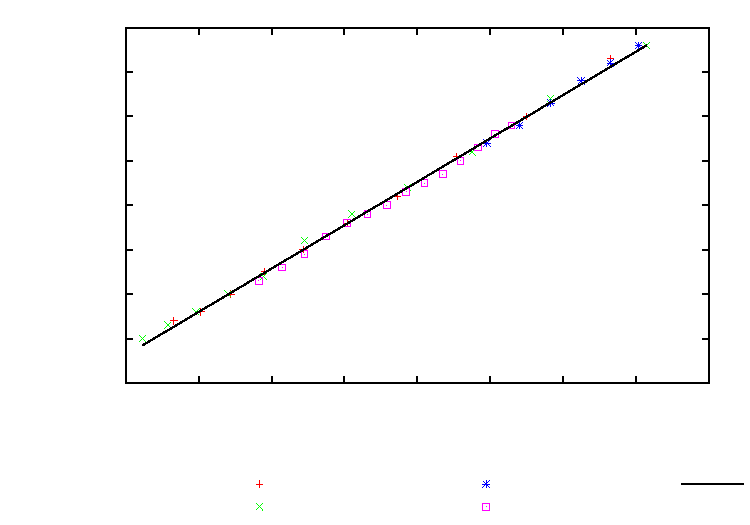
\includegraphics{UI}}%
    \gplfronttext
  \end{picture}%
\endgroup

	\caption{Durchmesser des Kreises gegen $\sqrt{\frac{U_\text{B}}{1\text V}}/\frac{I_\text{H}}{1\text A}$}
	\label{fig:UI}
\end{figure}
In Abb. \ref{fig:UI} erkennt man einen linearen Zusammenhang.
Dieser sollte sich auch nach Gleichung \eqref{eq:ui} ergeben.



\begin{table}[h!]
	\centering
	\begin{tabular}{|l|l|l|l|}
		 \hline
		 Spannung $U_B$\;[V] & Strom $I$\;[100 mA] & Radius $r$\;[mm] & $e/m_e$\;[$10^{11}\;$C\;kg$^{-1}$]\\
		 \hline
		 $120,0 \pm 0,5$ & $7,0 \pm 0,1$& $36,5 \pm 0,4$ & $1,78 \pm 0,06$\\
		 \hline                         
		 $130,0 \pm 0,5$ & $7,0 \pm 0,1$& $38,0 \pm 0,4$ & $1,78 \pm 0,06$\\
		 \hline                         
		 $140,0 \pm 0,5$ & $7,0 \pm 0,1$& $39,5 \pm 0,4$ & $1,77 \pm 0,06$\\
		 \hline                         
		 $150,0 \pm 0,5$ & $7,0 \pm 0,1$& $41,5 \pm 0,4$ & $1,72 \pm 0,06$\\
		 \hline                         
		 $160,0 \pm 0,5$ & $7,0 \pm 0,1$& $43,0 \pm 0,4$ & $1,71 \pm 0,06$\\
		 \hline                         
		 $170,0 \pm 0,5$ & $7,0 \pm 0,1$& $44,0 \pm 0,4$ & $1,73 \pm 0,06$\\
		 \hline                         
		 $180,0 \pm 0,5$ & $7,0 \pm 0,1$& $45,0 \pm 0,4$ & $1,75 \pm 0,06$\\
		 \hline                         
		 $190,0 \pm 0,5$ & $7,0 \pm 0,1$& $46,5 \pm 0,4$ & $1,73 \pm 0,06$\\
		 \hline                         
		 $200,0 \pm 0,5$ & $7,0 \pm 0,1$& $47,5 \pm 0,4$ & $1,75 \pm 0,06$\\
		 \hline                         
		 $210,0 \pm 0,5$ & $7,0 \pm 0,1$& $48,5 \pm 0,4$ & $1,76 \pm 0,06$\\
		 \hline                         
		 $220,0 \pm 0,5$ & $7,0 \pm 0,1$& $50,0 \pm 0,4$ & $1,74 \pm 0,06$\\
		 \hline                         
		 $230,0 \pm 0,5$ & $7,0 \pm 0,1$& $51,5 \pm 0,4$ & $1,71 \pm 0,06$\\
		 \hline                         
		 $240,0 \pm 0,5$ & $7,0 \pm 0,1$& $53,0 \pm 0,4$ & $1,68 \pm 0,05$\\
		 \hline                         
		 $250,0 \pm 0,5$ & $7,0 \pm 0,1$& $54,0 \pm 0,4$ & $1,69 \pm 0,05$\\
		 \hline                         
		 $120,0 \pm 0,5$ & $5,0 \pm 0,1$& $52,0 \pm 0,4$ & $1,72 \pm 0,07$\\
		 \hline                         
		 $130,0 \pm 0,5$ & $5,0 \pm 0,1$& $54,0 \pm 0,4$ & $1,72 \pm 0,07$\\
		 \hline                         
		 $140,0 \pm 0,5$ & $5,0 \pm 0,1$& $56,5 \pm 0,4$ & $1,70 \pm 0,07$\\
		 \hline                         
		 $150,0 \pm 0,5$ & $5,0 \pm 0,1$& $59,0 \pm 0,4$ & $1,67 \pm 0,07$\\
		 \hline                         
		 $160,0 \pm 0,5$ & $5,0 \pm 0,1$& $61,0 \pm 0,4$ & $1,66 \pm 0,07$\\
		 \hline                         
		 $170,0 \pm 0,5$ & $5,0 \pm 0,1$& $63,0 \pm 0,4$ & $1,66 \pm 0,07$\\
		 \hline                         
		 $140,0 \pm 0,5$ & $4,5 \pm 0,1$& $63,0 \pm 0,4$ & $1,68 \pm 0,08$\\
		 \hline                         
		 $140,0 \pm 0,5$ & $5,0 \pm 0,1$& $57,0 \pm 0,4$ & $1,67 \pm 0,07$\\
		 \hline                         
		 $140,0 \pm 0,5$ & $5,5 \pm 0,1$& $51,0 \pm 0,4$ & $1,72 \pm 0,07$\\
		 \hline                         
		 $140,0 \pm 0,5$ & $6,0 \pm 0,1$& $47,0 \pm 0,4$ & $1,70 \pm 0,06$\\
		 \hline                         
		 $140,0 \pm 0,5$ & $6,5 \pm 0,1$& $44,0 \pm 0,4$ & $1,65 \pm 0,06$\\
		 \hline                         
		 $140,0 \pm 0,5$ & $7,0 \pm 0,1$& $41,0 \pm 0,4$ & $1,64 \pm 0,06$\\
		 \hline                         
		 $140,0 \pm 0,5$ & $7,5 \pm 0,1$& $37,0 \pm 0,4$ & $1,76 \pm 0,06$\\
		 \hline                         
		 $140,0 \pm 0,5$ & $8,0 \pm 0,1$& $35,0 \pm 0,4$ & $1,73 \pm 0,06$\\
		 \hline                         
		 $140,0 \pm 0,5$ & $8,5 \pm 0,1$& $33,0 \pm 0,4$ & $1,72 \pm 0,06$\\
		 \hline                         
		 $140,0 \pm 0,5$ & $9,0 \pm 0,1$& $31,5 \pm 0,4$ & $1,68 \pm 0,06$\\
		 \hline                         
		 $140,0 \pm 0,5$ & $9,5 \pm 0,1$& $30,0 \pm 0,4$ & $1,67 \pm 0,06$\\
		 \hline                         
		 $160,0 \pm 0,5$ & $5,0 \pm 0,1$& $61,5 \pm 0,4$ & $1,64 \pm 0,07$\\
		 \hline                         
		 $160,0 \pm 0,5$ & $5,5 \pm 0,1$& $55,0 \pm 0,4$ & $1,69 \pm 0,07$\\
		 \hline                         
		 $160,0 \pm 0,5$ & $6,0 \pm 0,1$& $50,5 \pm 0,4$ & $1,68 \pm 0,06$\\
		 \hline                         
		 $160,0 \pm 0,5$ & $6,5 \pm 0,1$& $46,0 \pm 0,4$ & $1,73 \pm 0,06$\\
		 \hline                         
		 $160,0 \pm 0,5$ & $7,0 \pm 0,1$& $43,0 \pm 0,4$ & $1,71 \pm 0,06$\\
		 \hline                         
		 $160,0 \pm 0,5$ & $7,5 \pm 0,1$& $40,0 \pm 0,4$ & $1,72 \pm 0,06$\\
		 \hline                         
		 $160,0 \pm 0,5$ & $8,0 \pm 0,1$& $37,5 \pm 0,4$ & $1,72 \pm 0,06$\\
		 \hline                         
		 $160,0 \pm 0,5$ & $8,5 \pm 0,1$& $35,0 \pm 0,4$ & $1,75 \pm 0,06$\\
		 \hline                         
		 $160,0 \pm 0,5$ & $9,0 \pm 0,1$& $33,0 \pm 0,4$ & $1,75 \pm 0,06$\\
		 \hline                         
		 $160,0 \pm 0,5$ & $9,5 \pm 0,1$& $32,0 \pm 0,4$ & $1,67 \pm 0,05$\\
		  \hline
	  \end{tabular}
	  \caption{Messreihen}
	  \label{tbl:pythonmessung}
  \end{table}
Insgesamt ergibt sich aus der Tabelle \ref{tbl:pythonmessung} ein gewichteter Mittelwert von $(1.7104 \pm 0.0096)\si{\coulomb/\kilo\gram}$ über alle Messungen.
Dies ergibt eine Abweichung vom Literaturwert $1.7588\si{\coulomb/\kilo\gram}$ von $3\%$

\begin{figure}[!h]
	\centering
	% GNUPLOT: LaTeX picture with Postscript
\begingroup
  \makeatletter
  \providecommand\color[2][]{%
    \GenericError{(gnuplot) \space\space\space\@spaces}{%
      Package color not loaded in conjunction with
      terminal option `colourtext'%
    }{See the gnuplot documentation for explanation.%
    }{Either use 'blacktext' in gnuplot or load the package
      color.sty in LaTeX.}%
    \renewcommand\color[2][]{}%
  }%
  \providecommand\includegraphics[2][]{%
    \GenericError{(gnuplot) \space\space\space\@spaces}{%
      Package graphicx or graphics not loaded%
    }{See the gnuplot documentation for explanation.%
    }{The gnuplot epslatex terminal needs graphicx.sty or graphics.sty.}%
    \renewcommand\includegraphics[2][]{}%
  }%
  \providecommand\rotatebox[2]{#2}%
  \@ifundefined{ifGPcolor}{%
    \newif\ifGPcolor
    \GPcolortrue
  }{}%
  \@ifundefined{ifGPblacktext}{%
    \newif\ifGPblacktext
    \GPblacktexttrue
  }{}%
  % define a \g@addto@macro without @ in the name:
  \let\gplgaddtomacro\g@addto@macro
  % define empty templates for all commands taking text:
  \gdef\gplbacktext{}%
  \gdef\gplfronttext{}%
  \makeatother
  \ifGPblacktext
    % no textcolor at all
    \def\colorrgb#1{}%
    \def\colorgray#1{}%
  \else
    % gray or color?
    \ifGPcolor
      \def\colorrgb#1{\color[rgb]{#1}}%
      \def\colorgray#1{\color[gray]{#1}}%
      \expandafter\def\csname LTw\endcsname{\color{white}}%
      \expandafter\def\csname LTb\endcsname{\color{black}}%
      \expandafter\def\csname LTa\endcsname{\color{black}}%
      \expandafter\def\csname LT0\endcsname{\color[rgb]{1,0,0}}%
      \expandafter\def\csname LT1\endcsname{\color[rgb]{0,1,0}}%
      \expandafter\def\csname LT2\endcsname{\color[rgb]{0,0,1}}%
      \expandafter\def\csname LT3\endcsname{\color[rgb]{1,0,1}}%
      \expandafter\def\csname LT4\endcsname{\color[rgb]{0,1,1}}%
      \expandafter\def\csname LT5\endcsname{\color[rgb]{1,1,0}}%
      \expandafter\def\csname LT6\endcsname{\color[rgb]{0,0,0}}%
      \expandafter\def\csname LT7\endcsname{\color[rgb]{1,0.3,0}}%
      \expandafter\def\csname LT8\endcsname{\color[rgb]{0.5,0.5,0.5}}%
    \else
      % gray
      \def\colorrgb#1{\color{black}}%
      \def\colorgray#1{\color[gray]{#1}}%
      \expandafter\def\csname LTw\endcsname{\color{white}}%
      \expandafter\def\csname LTb\endcsname{\color{black}}%
      \expandafter\def\csname LTa\endcsname{\color{black}}%
      \expandafter\def\csname LT0\endcsname{\color{black}}%
      \expandafter\def\csname LT1\endcsname{\color{black}}%
      \expandafter\def\csname LT2\endcsname{\color{black}}%
      \expandafter\def\csname LT3\endcsname{\color{black}}%
      \expandafter\def\csname LT4\endcsname{\color{black}}%
      \expandafter\def\csname LT5\endcsname{\color{black}}%
      \expandafter\def\csname LT6\endcsname{\color{black}}%
      \expandafter\def\csname LT7\endcsname{\color{black}}%
      \expandafter\def\csname LT8\endcsname{\color{black}}%
    \fi
  \fi
  \setlength{\unitlength}{0.0500bp}%
  \begin{picture}(7200.00,5040.00)%
    \gplgaddtomacro\gplbacktext{%
      \csname LTb\endcsname%
      \put(1078,1584){\makebox(0,0)[r]{\strut{} 1.55}}%
      \put(1078,2116){\makebox(0,0)[r]{\strut{} 1.6}}%
      \put(1078,2648){\makebox(0,0)[r]{\strut{} 1.65}}%
      \put(1078,3180){\makebox(0,0)[r]{\strut{} 1.7}}%
      \put(1078,3711){\makebox(0,0)[r]{\strut{} 1.75}}%
      \put(1078,4243){\makebox(0,0)[r]{\strut{} 1.8}}%
      \put(1078,4775){\makebox(0,0)[r]{\strut{} 1.85}}%
      \put(1210,1364){\makebox(0,0){\strut{} 0.06}}%
      \put(2009,1364){\makebox(0,0){\strut{} 0.07}}%
      \put(2808,1364){\makebox(0,0){\strut{} 0.08}}%
      \put(3607,1364){\makebox(0,0){\strut{} 0.09}}%
      \put(4406,1364){\makebox(0,0){\strut{} 0.1}}%
      \put(5205,1364){\makebox(0,0){\strut{} 0.11}}%
      \put(6004,1364){\makebox(0,0){\strut{} 0.12}}%
      \put(6803,1364){\makebox(0,0){\strut{} 0.13}}%
      \put(176,3179){\rotatebox{-270}{\makebox(0,0){\strut{}$e/m_e$ [$10^{11}$C/kg]}}}%
      \put(4006,1034){\makebox(0,0){\strut{}Bahndurchmesser [m]}}%
    }%
    \gplgaddtomacro\gplfronttext{%
      \csname LTb\endcsname%
      \put(3151,613){\makebox(0,0)[r]{\strut{}I=0.5A}}%
      \csname LTb\endcsname%
      \put(3151,393){\makebox(0,0)[r]{\strut{}I=0.7A}}%
      \csname LTb\endcsname%
      \put(3151,173){\makebox(0,0)[r]{\strut{}U=140V}}%
      \csname LTb\endcsname%
      \put(5722,613){\makebox(0,0)[r]{\strut{}U=160V}}%
      \csname LTb\endcsname%
      \put(5722,393){\makebox(0,0)[r]{\strut{}Literaturwert}}%
    }%
    \gplbacktext
    \put(0,0){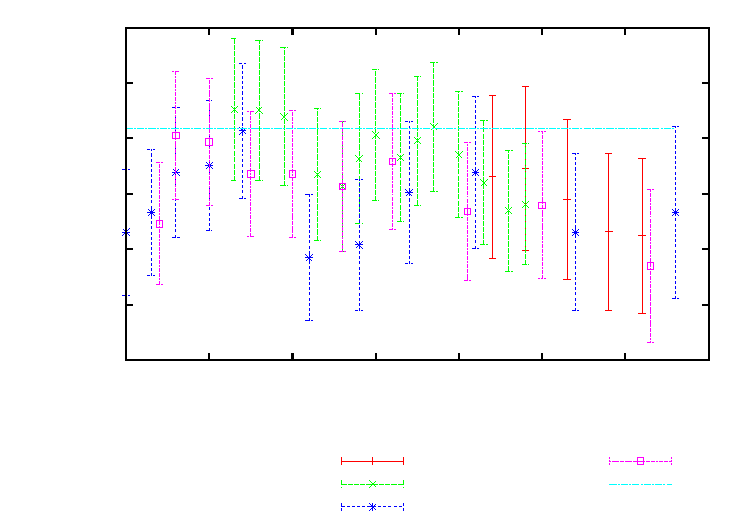
\includegraphics{eric}}%
    \gplfronttext
  \end{picture}%
\endgroup

	\caption{Durchmesser des Kreises gegen $\sqrt{\frac{U_\text{B}}{1\text V}}/\frac{I_\text{H}}{1\text A}$}
	\label{fig:eric}
\end{figure}


\section{Diskussion}
\label{sec:diskussion}

\bibliography{literatur}
\end{document}
